\documentclass[11pt]{article}
\usepackage{amsmath, amssymb, amsfonts, amsthm, graphicx}
\setlength{\parindent}{0pt}

\newcommand{\nc}{\newcommand}
\nc{\x}{\tau_{0}}
\nc{\y}{\tau_{2}}
\nc{\z}{\tau_{1}}


\theoremstyle{plain}
\newtheorem{theorem}{Theorem}[section]
\newtheorem{lemma}[theorem]{Lemma}
\newtheorem{proposition}[theorem]{Proposition}

\theoremstyle{definition}
\newtheorem{definition}[theorem]{Definition}
\newtheorem{corollary}[theorem]{Corollary}
\newtheorem{notation}[theorem]{Notation}
\newtheorem{example}[theorem]{Example}

\begin{document}
\title{Three-period orbits in billiards on the surfaces of constant curvature}
\author{V. Blumen., K. Y. Kim, N. K., J. Nance, and V. Zharnitsky}
\maketitle

\begin{abstract}
In the spirit of Wojtkowski's paper, we present proofs that there are no open sets of three-period orbits in hyperbolic
 or spherical billiards. Rather than using variational methods as is standard for these types of billiards problems,
 our approach is differential geometric, using Jacobi fields to analyze two-parameter families of nearby orbits.
\end{abstract}
\tableofcontents
\section{Introduction}
This article provides a unified approach to study open sets of 3-period orbits in billiards on manifolds with constant curvature. Specifically, Euclidean, spherical and hyperbolic have been treated. Although Euclidean and spherical have been treated previously, we offer new results on the hyperbolic case. Open sets, or rather sets of positive measure, of periodic orbits is important in spectral asymptotics for the corresponding eigenvalue problem. Understanding the structure of periodic orbits in non-Euclidean geometries might also help our understanding of the planar case.

The billiard system on a two dimensional Riemannian manifold $(M,g)$ consists of the boundary $\partial Q$ and
a mass point moving along the geodesics inside the domain. Whenever the mass hits the boundary, it reflects
according to the Fermat's principle so as to extremize the path length, which in turn leads to the familiar law:
the angle of incidence  is equal to the angle of reflection. Even more general formulation is possible in the
framework  of Finsler geometry, see \cite{tabachnikov_finsler}.

Periodic orbits is a natural object of study in dynamical systems and one important question concerns
the presence of ``large'' sets (of positive measure) of periodic orbits in the billiard ball problem. Informally speaking,
it corresponds to the probability that a given orbit is periodic.
This question has been originally motivated by the spectral geometry problem. It turns out that the second term
of the so-called Weyl asymptotics for, say, the Dirichlet problem in a bounded domain has a particularly simple
 form if periodic orbits the associated billiard problem has zero measure \cite{ivrii}. There is a natural invariant
 measure for the billiard map which can be defined as follows:
let $s$ be an arclength parameter coordinatizing the boundary and let
$\phi \in [0,\pi]$ be the angle of the outcoming ray from the boundary measured in the counterclockwise direction.

The billiard ball map $T: [\partial Q\times [0,\pi]] \rightarrow Q\times [0,\pi]]$ which takes one outcoming ray to
another one obtained after reflection from the boundary, preserves the measure $\mu = \sin \phi\, d\phi \, ds$, see e.g.
\cite{birkhoff}.

Regarding motivations, we finally mention that understanding the structure of periodic orbits in non-Euclidean geometries
might also help our understanding of the planar case. It is also likely that spectral geometry in non-Euclidean
geometries would also require understanding the structure of the the sets of periodic orbits.


For the planar (classical) billiard problem, it is easy to see that two period orbits have zero measure,
since they must be normal to the boundary at both ends. Similarly, this is the case for a billiard on ${\mathbb H^2}$.
On the other hand, a billiard on $S^2$ with boundary given by equator has two-period orbits of positive (in fact, full)
measure. This has to do with the presence of conjugated points on $S^2$.

For the period 3, this problem already becomes non-trivial. First result on zero measure of 3-periodic orbit was
obtained by Rychlik in \cite{rychlik}, using symbolic calculations, which were later removed in \cite{stojanov}.
 Using Jacobi fields, Wojtkovski provided an elegant simple proof of Rychlik's theorem. Subsequently, there have been
extensions to other types of billiard systems: higher dimensional (\cite{vorobets}),
outer billiards (\cite{genin,tumanov}), and spherical (\cite{ymb}).

The purpose of this article is twofold. First we prove,

\begin{theorem}
The set of 3-period orbits in any billiard on ${\mathbb H^2}$ has zero measure.
\end{theorem}

Secondly, we present the unified proof (following Wojtkovski) based on the Jacobi fields,
which treats all 3 billiard systems on the constant curvature manifolds in the same manner.
Our argument proceeds independently of the underlying geometry until we get the compatibility
condition. Then, using the relevant cosine formula (which depends on the geometry), we obtain
the relation that must be satisfied at an open set containing only 3-period orbits
\[
k(s_0) =  \sin^3 (\phi_0)F(L),
\]
where $k(s_0)$ is curvature at one of the vertices and $\phi_0$ is the angle of the billiard orbit with tangent at this vertex.
The function $F(L)$ depends on the underlying Riemannian manifold
\[
 F(L) =
  \begin{cases}
   \frac{2}{L} & \text{if }  {\mathbb E^2} \\
   \coth(L/2)    & \text{if } {\mathbb H^2}  \\
   \cot(L/2)    & \text{if }  {\mathbb S^2}.
  \end{cases}
\]

From this formula, it is possible to classify sets of 3-period orbits.

\subsection{Notation}


\section{Billiard system on the surface of constant curvature}
\subsection{Jacobi fields}
Let $\mathcal{Q}$ be a smooth and convex domain on a surface of constant curvature $\kappa$. The billiard ball travels along the geodesics inside $\mathcal{Q}$ and reflects at the boundary. We represent a two parameter family of billiard orbits by $\gamma(\epsilon, \tau),$  where $|\epsilon| < \epsilon_0, -\infty < \tau < \infty$. \\

The Jacobi field $J(\tau)$ is defined as\\
\[
\displaystyle J(\tau)=\frac{\partial \gamma(0, \tau)}{\partial \epsilon}.
\]
It describes the behavior of nearby orbits and satisfies the Jacobi equation
\[\displaystyle \frac{D^2}{d^2\tau}J(\tau)+ \kappa J(\tau) =0\]
where D denotes the covariant derivative. Since the Jacobi equation is a second order linear differential equation, we get a unique solution if two initial conditions $J(0)$ and  $J'(0)$  are given. \\

\subsection{Collision and reflection matrices}

We focused on the billiards on the hyperbolic 2-space and the 2-sphere which have the sectional curvature $\kappa =1$ and $-1$ respectively.  We solved the Jacobi equation to get

\[
J(\tau)=\left\{ \begin{array}{cl}
J(0) \cosh(\tau)+J'(0) \sinh(\tau)& $if $\mathbb{H}^2 \\
J(0)\cos(\tau) + J'(0)\sin(\tau)& $if $\mathbb{S}^2\\
 \end{array} \right.
\]
Differentiating with respect to $\tau$ gives us

\[
J'(\tau)=\left\{ \begin{array}{cl}
J(0) \sinh(\tau)+J'(0) \cosh(\tau)& $if $\mathbb{H}^2 \\
-J(0)\sin(\tau) + J'(0)\cos(\tau)\,\,\,\,& $if $\mathbb{S}^2\\
 \end{array} \right.
\]

In each case, we construct the Collision matrix $C(\tau)$,
\[
\left( \begin{array}{c}
J(\tau) \\
J'(\tau) \\
 \end{array} \right)
= C(\tau)
\left( \begin{array}{c}
J(0) \\
J'(0) \\
 \end{array} \right)
\]

which describes the evolution of a Jacobi field over time.\\


When the ball hits the boundary at $x=(s, \phi)$, the Jacobi field changes by the linear map $R(x)$
\[
\left( \begin{array}{r}
J_{out} \\
J'_{out} \\
 \end{array} \right)
=R(x)
 \left( \begin{array}{r}
J_{in} \\
J'_{in} \\
 \end{array} \right)
\]


Now let us consider 3-period orbits with $x_0, x_1$ and $x_2$ as the collision points. Then we must have $T^3$ equal to identity, that is
\[
C(\x)R(x_0)C(\z) = R^{-1}(x_1)C^{-1}(\y)R^{-1}(x_2).
\]
We denote $\x$ the time for the billiard ball to reach the next boundary point after the boundary point $x_0$.


\section{Billiard on hyperbolic plane}
\begin{center}
    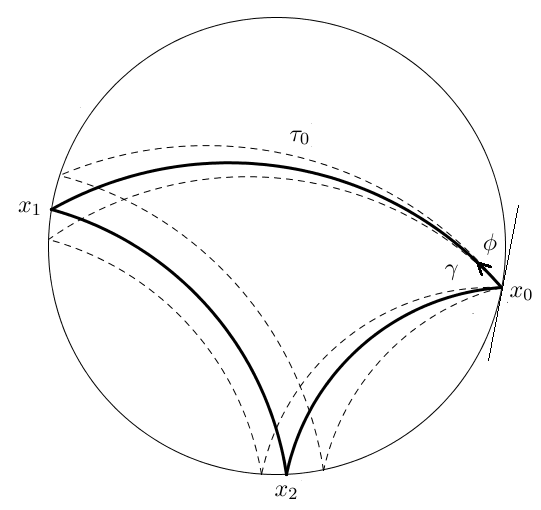
\includegraphics[width=.5\textwidth]{hyperbolic.png}
 \end{center}


\subsection{Collision and reflection matrices in hyperbolic billiards}
\subsection{The main result for the hyperbolic case}
\begin{definition}
\textit{The following relation holds when $\gamma$ is the angle subtending from two adjacent segments of an orbit and $\phi$ is the angle of incidence (reflection): $\sin(\phi)=\sin(\frac{\pi-\gamma}{2})=\cos(\frac{\gamma}{2})$.
The length of an orbit is given by $L:=\x+\y+\x$.}
\end{definition}
The collision and reflection matrices describing evolution of an orbit are given respectively as
\begin{equation*}
C(\x)=\left(\begin{array}{cc}
\cosh(\x) & \sinh(\x) \\
\sinh(\x) & \cosh(\x) \end{array}\right)
\mbox{ and }
R(\x)=\left(\begin{array}{cc}
-1 & 0 \\
\frac{2k_0}{\sin(\phi)} & -1 \end{array}\right).
\end{equation*}
Now a single orbit can be realized as the product of six matrices,
\begin{equation*}
C(\x)R(\x)C(\z)\left(\begin{array}{c}
0 \\
1\end{array}\right)=R^{-1}(\y)C^{-1}(\y)R^{-1}(\z)\left(\begin{array}{c}
0 \\
1\end{array}\right).
\end{equation*}

Equating components of the resulting vectors, we have

\begin{equation*}
  \sinh(\x+\z)-\sinh(\y)=\frac{2k_0\sinh(\x)\sinh(\z)}{\sin(\phi)}
\end{equation*}

\begin{equation*}
\cosh(\y)=\cosh(\x)\cosh(\z)-\sinh(\x)\sinh(\z)\cos(\gamma)
\end{equation*}

Simplify using the hyperbolic cosine angle addition formula to get

\begin{equation*}
\cosh(\y)=\cosh(\x+\z)-\sinh(\x)\sinh(\z)-\sinh(\x)\sinh(\z)\cos(\gamma).
\end{equation*}
Factoring, we arrive at
\begin{equation*}
\cosh(\x+\z)-\cosh(\y)=2 \cos^2(\frac{\gamma}{2})\sinh(\x)\sinh(\z)
\end{equation*}
Combining the results above,
\begin{equation*}
\frac{\cosh(\x+\z)-\cosh(\y)}{\cos^2(\frac{\gamma}{2})}=2\sinh(\x)\sinh(\z)=\frac{\sinh(\x+\z)-\sinh(\y)\cos(\frac{\gamma}{2})}{k_0}.
\end{equation*}
Therefore,
\begin{equation*}
k_0=\frac{\sinh(\x+\z)-\sinh(\y)}{\cosh(\x+\z)-\cosh(\y)}\cos^3(\frac{\gamma}{2})
\end{equation*}
Exploiting identities for $\sinh(A)-\sinh(B)$ and $\cosh(A)-\cosh(B)$, we can conclude that

\begin{equation*}\begin{split}
k_0&=\frac{\sinh(L-\y)-\sinh(\y)}{\cosh(L-\y)-\cosh(\y)}\cos^3(\frac{\gamma}{2}) \\
&=\frac{2\cosh(L/2)\sinh(L/2-\y)}{2\sinh(L/2)\sinh(L/2-\y)}\cos^3(\frac{\gamma}{2}) \\
&=\cos^3(\frac{\gamma}{2})\cdot\mbox{ constant}\end{split}
\end{equation*}


\section{Spherical billiard}
\begin{center}
    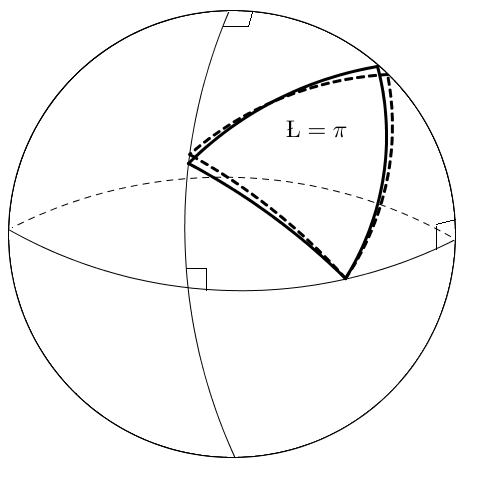
\includegraphics[width=.5\textwidth]{spherical.png}
 \end{center}


\subsection{Collision and reflection matrices in spherical billiards}
\subsection{Special case}
Equating the components of the resulting vectors,


\begin{equation*}
\frac{2k_0\sin(\x)\sin(\z)}{\sin(\phi)}=\sin(\x)\cos(\z)+\cos(\x)\sin(\z)-\sin(\y).
\end{equation*}

Using the sine and cosine angle addition formulae,


\begin{equation*}
\frac{2k_0\sin(\x)\sin(\z)}{\sin(\phi)}=\sin(\x+\z)-\sin(\y).
\end{equation*}
The fact that
\begin{equation*}
\cos(\y)=\cos(\x)\cos(\z)+\sin(\x)\sin(\z)\cos(\gamma)
\end{equation*}
allows us to write

\begin{equation*}\begin{split}
\cos(\x+\z)-\cos(\y)&=-(\sin(\x)\sin(\z)+\sin(\x)\sin(\z)\cos(\gamma)) \\
&=-(1+\cos(\gamma))\sin(\x)\sin(\z).
\end{split}
\end{equation*}
Using the cosine half-angle identity,

\begin{equation*}
\cos(\x+\z)-\cos(\y)=-2\cos^2(\frac{\gamma}{2})\sin(\x)\sin(\z)
\end{equation*}
can be written as

\begin{equation*}
\frac{k_0}{\cos(\frac{\gamma}{2})}\left(\frac{-\cos(\x+\z)-\cos(\y)}{\cos^2(\frac{\gamma}{2})} \right)=\sin(\x+\z)-\sin(\y).
\end{equation*}
Therefore,

\begin{equation*}
k_0=-\left( \frac{\sin(\x+\z)-\sin(\y)}{\cos(\x+\z)-\cos(\y)}\right)\cos^3(\frac{\gamma}{2}).
\end{equation*}
Exploiting identities for $\sin(A)\pm \sin(B)$ and $\cos(A)\pm\cos(B)$, we can write
\begin{equation*}
k_0=-\cos^3(\frac{\gamma}{2})\left(\frac{2\cos(\frac{\x+\y+\z}{2})\sin(\frac{\x+\z-\y}{2})}{-2\sin(\frac{\x+\y+\z}{2})\sin(\frac{\x+\z-\y}{2})} \right).
\end{equation*}

Therefore,

\begin{equation*}
k_0=\cos^3(\frac{\gamma}{2})\cdot \mbox{constant}
\end{equation*}

a contradiction if $L\neq n \pi$ for $n$ odd.
\newline

Notice that if $L=\pi,\ 3\pi, 5\pi,\ldots$, then $k_0=0=\mbox{constant}$ which does not contradict our assertion that $k_0=constant$. This means that the boundary $\partial Q$ has zero geodesic curvature, so the boundary itself is comprised of geodesics on the sphere. This means that if in unit-spherical billiards, the length of a three-period orbit is equal to an odd multiple of $\pi$, then you are guaranteed to have an open set of three-period orbits. One can convince oneself by a simple reflection argument as follows: ?????????


\section{Conclusions}
\section{Acknowledgements}

\begin{thebibliography}{100}
\bibitem{ymb} Y.M. Baryshnikov, Spherical billiards with periodic orbits, preprint.
\bibitem{birkhoff} G.D. Birkhoff, Dynamical Systems,
\bibitem{genin} D. Genin, S. Tabachnikov. On configuration space of plane polygons, sub-Riemannian geometry
and periodic orbits of outer billiards. J. Modern Dynamics, 1 (2007), 155-173.
\bibitem{tumanov} A. Tumanov and V. Zharnitsky, Periodic orbits in outer billiard, International Mathematics Research Notices, vol. 2006, 1-17.
\bibitem{rychlik} M. R. Rychlik, Periodic points of the billiard ball map in a convex domain, Journal of Differential Geometry 30 (1989), no. 1, 191-205.
\bibitem{stojanov} L. Stojanov, Note on the periodic points of the billiard, Journal of Differential Geometry 34 (1991), no. 3, 835-837.
\bibitem{wojtk} M. P. Wojtkowski, Two applications of Jacobi fields to the billiard ball problem, Journal of Differential Geometry 40 (1994), no. 1, 155-164.
\bibitem{tabachnikov_finsler} E. Gutkin, S. Tabachnikov. Billiards in Finsler and Minkowski geometries. J. Geom. and Phys., 40 (2002), 277.
\bibitem{ivrii} V. Ya. Ivrii, The second term of the spectral asymptotics for a laplace-beltrami operator on manifolds with boundary, Func. Anal. Appl. 14 (2) (1980), 98–106.
\bibitem{vorobets} Ya. B. Vorobets, On the measure of the set of periodic points of a billiard, Mathematical Notes 55(1994), no. 5, 455-460.
\bibitem{jml} J. M. Landsberg, Exterior differential systems and billiards, Proceedings of the 7th International Conference on Geometry, Integrability and Quantization held in Varna, 2005, Softex, Sofia, pp. 35-54.

\end{thebibliography}

\end{document} 